\documentclass{article}
\usepackage[utf8]{inputenc}
\usepackage[english]{babel}
\usepackage[]{amsthm} %lets us use \begin{proof}
\usepackage[]{amssymb} %gives us the character \varnothing
\usepackage[]{setspace} %provides commands to set line spacing
\usepackage[left=0.75in, right=0.75in]{geometry}
\usepackage{hyperref}
\usepackage{xcolor}
\usepackage{amsmath}
\usepackage{enumitem}
\usepackage{graphicx}
\usepackage{subfigure}
\usepackage{float}
\usepackage{soul}

\geometry{a4paper, margin=1in}


\begin{document}

\begin{center}
	\LARGE{Finite Potential Well}\\[1em]
	\large Son [Joe] Nguyen\\[1em]
	%\large \today
\end{center}

\subsection*{Finite Square Well}
The finite square well is a potential energy function that is defined piecewise as follows:
\begin{equation*}
    V(x) = \begin{cases}
        -V_0 & \text{if } -a \leq x \leq a,\\
        0 & \text{otherwise}.
    \end{cases}
\end{equation*}

\noindent The mass of $^{87}$Rb is $m = 1.443 \times 10^{-25}$ kg.
\[z_0 = \frac{a}{\hbar} \sqrt{2mV_0}\]

\noindent The condition for having three bound states corresponds to \(z_0\) lying within a range that supports
exactly three bound energy levels. The range is given by the following inequality: 
\[\pi < z_0 < \frac{3 \pi}{2} \] 

\noindent Let choose \(a = 1nm =  1 \cdot 10^{-9}\) m and \(z_0 = 4\). We can calculate the value of \(V_0\) that satisfies the condition
for having three bound states. We can reagrange the equation to solve for \(V_0\):

\[|V_0| =  \frac{(z_0)^2 \hbar^2}{2ma^2} = \frac{\left(4\right)^2 (1.055 \cdot 10^{-34})^2}{2 (1.443 \cdot 10^{-25}) (1 \cdot 10^{-9})^2} \approx 6.1706 \cdot 10^{-25} J \approx 3.8514 \cdot 10^{-6}eV\]
\\ 

\noindent Where \(a\) is half-width of the Well. 
\\ \\
\noindent \hl{In the region of $x < -a$, the potential is zero, we have the Shrodinger equation:}

\begin{equation}
    - \frac{\hbar^2}{2m} \frac{d^2 \psi}{d x^2} = E \psi, \, \text{or} \, \frac{d^2 \psi}{d x^2} = \kappa^2 \psi
\end{equation}
Where: \(\kappa \equiv \frac{\sqrt{-2mE}}{\hbar}\)
\begin{equation}
    \psi_1 = Ae^{\kappa x}
\end{equation}

\noindent \hl{ In the region of $-a \leq x \leq a$:}
\begin{equation}
    - \frac{\hbar^2}{2m} \frac{d^2 \psi}{d x^2} - V_0 \psi = E \psi,  \, \text{or} \, \frac{d^2 \psi}{d x^2} = - l^2 \psi
\end{equation}
Where: \(l \equiv \frac{\sqrt{2m(V_0 + E)}}{\hbar}\)
\begin{equation}
    \psi_2 = B \sin(l x) + C \cos(l x)
\end{equation}
\\ \\
\noindent \hl{In the region of $x > a$:} 
\begin{equation}
E \psi = -\frac{\hbar}{2m} \frac{d^2 \psi}{dx^2} \, \text{or} \, \frac{d^2 \psi}{dx^2} = \kappa^2 \psi
\end{equation}
\\ 
\begin{equation}
\psi_3 = De^{-\kappa x}
\end{equation}

\noindent For the even bound states:
\begin{equation}
    \label{eq:even}
    \psi(x) = \begin{cases}
        Ae^{\kappa x} & \text{if } x < -a,\\
        C \cos(l x) & \text{if } -a \leq x \leq a,\\
        De^{-\kappa x} & \text{if } x > a.
    \end{cases}
\end{equation}
It's transcendental equation is \(\tan(z) = \sqrt{\left(\frac{z_0}{z}\right)^2 -1}\)
where \(z = l a\) \\ \\
Plug in the constants, we have:
\begin{equation}
    z = la = \frac{\sqrt{2m(V_0 + E)}}{\hbar} a = \frac{\sqrt{2(1.443 \cdot 10^{-25})(6.1706 \cdot 10^{-25} J + E)}}{1.055\cdot 10^{-34} J} \cdot 10^{-9}
\end{equation}
\noindent For the odd bound states:
\begin{equation}    
    \psi(x) = \begin{cases}
        Ae^{\kappa x} & \text{if } x < -a,\\
        B \sin(l x) & \text{if } -a \leq x \leq a,\\
        De^{-\kappa x} & \text{if } x > a.
    \end{cases}
\end{equation}
It's transcendental equation is \(-\cot(z) = \sqrt{\left(\frac{z_0}{z}\right)^2 - 1}\)  \\ \\
The graph of even and odd bound states are shown below:
\begin{figure}[H]
    \centering
    \subfigure[Even and Odd Bound States]{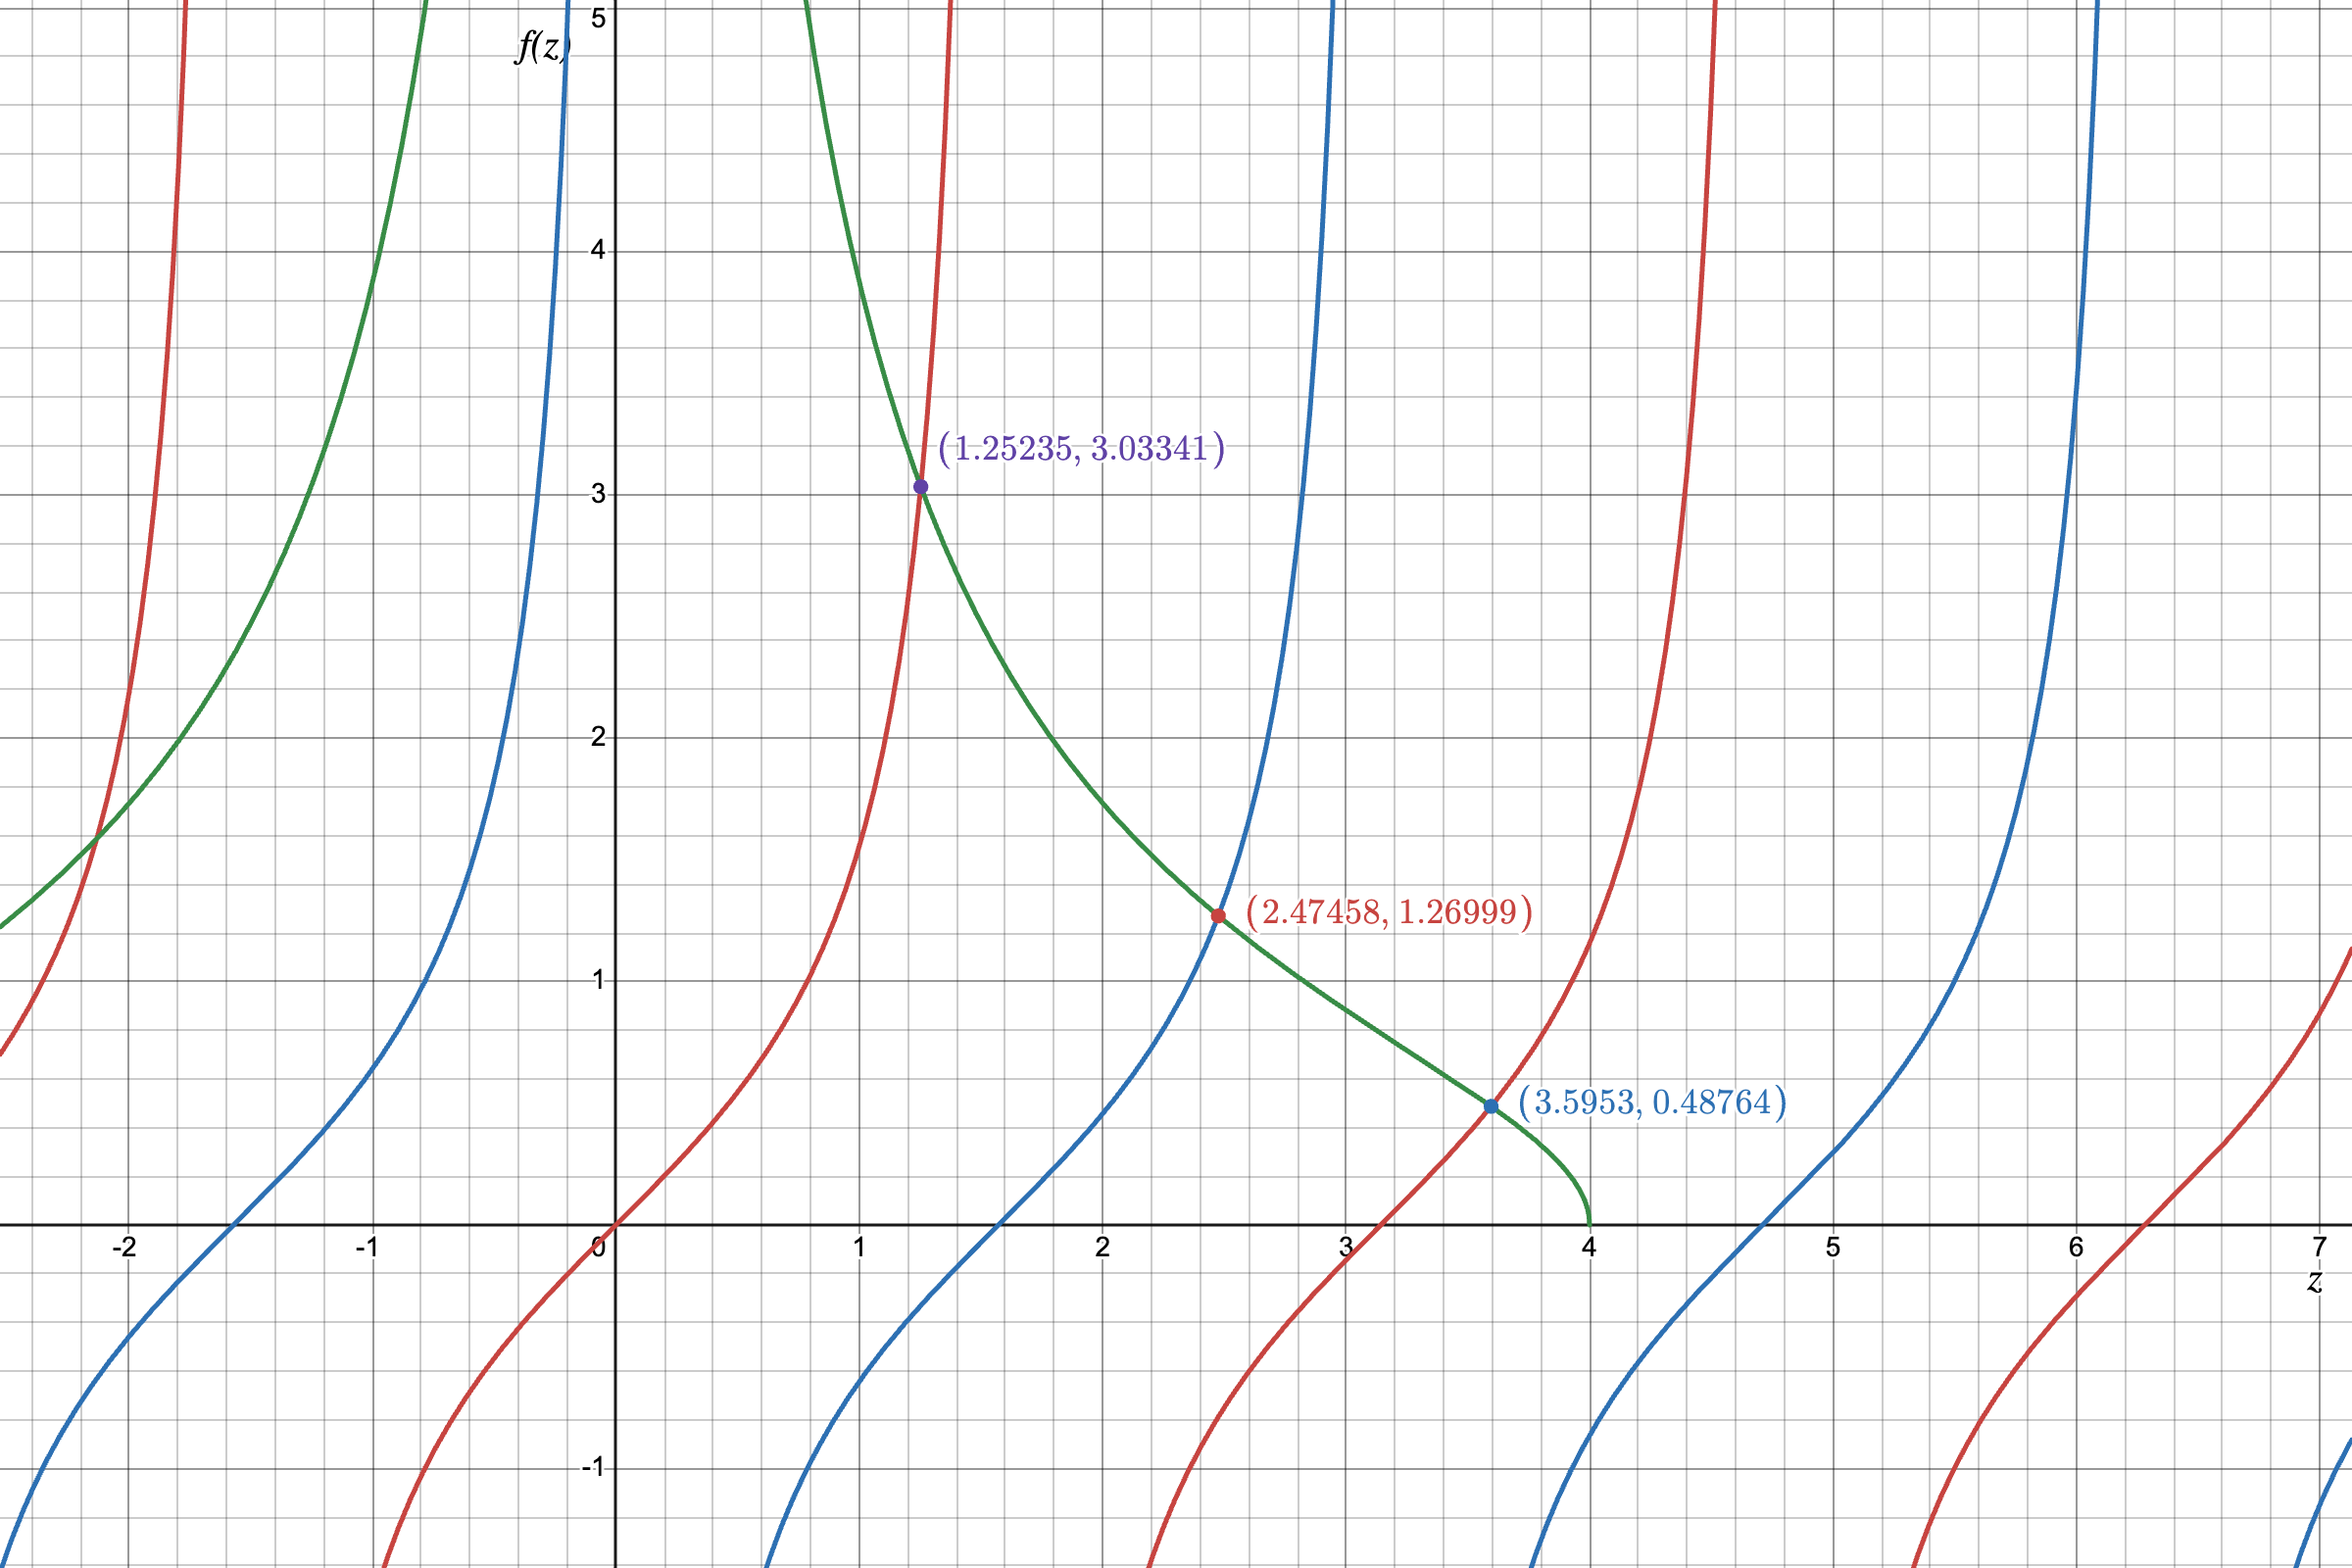
\includegraphics[width=0.45\textwidth]{evenodd.png}}
\end{figure}
The red line is the function of \(f(z) = \tan(z)\) and the blue line is the function of \(g(z) = -\cot(z)\), the green line is the function of \(h(z) = \sqrt{\left(\frac{4}{z}\right)^2}-1\) at \(z_0 = 4\). We can see there are 3 intersections
at \(z_0 = 1.25235 \, \text{(even)}, z_1 = 2.47458 \, \text{(odd)}, z_2 = 3.5953 \, \text{(even)} \). Plug in the value of \(z_n\) for equation (8). We can get the value of \(E_n\). 
\begin{align*}
    E_0 & \approx -5.57113 \cdot 10^{-25} \, (J), l_0 \approx 1.2523 \cdot 10^9 , \kappa_0 \approx 3.8 \cdot 10^9 \\
    E_1 & \approx  -3.80897 \cdot 10^{-25} \, (J), l_1 \approx 2.47458 \cdot 10^9, \kappa_1 \approx 3.14 \cdot 10^9\\
    E_2 & \approx -1.18544 \cdot 10^{-25} \, (J), l_2 \approx 3.5953 \cdot 10^9, \kappa_2 \approx 1.75 \cdot 10^9
\end{align*}
\\
Now we normalize the wave function for the even bound states to find the value of \(A, C, D\) from equation \eqref{eq:even}. We have:
\begin{align*}
    1 & = \int_{-\infty}^{\infty} |\psi(x)|^2 dx = \int_{-\infty}^{-a} |Ae^{\kappa x}|^2 dx + \int_{-a}^{a} |C \cos(l x)|^2 dx + \int_{a}^{\infty} |De^{-\kappa x}|^2 dx \\
    &= (A^2 + D^2)\int_{a}^{\infty} e^{-2kx} dx  + 2 C^2 \int_{0}^{a} \cos^2(lx) dx \\
    &= (A^2 + D^2)\frac{e^{-2\kappa a}}{2\kappa} +2 C^2 \left(\frac{2al + \sin(2al)}{4l}\right) \\
    &= (A^2 + D^2)\frac{e^{-2\kappa a}}{2\kappa} + C^2 \left(a + \frac{\sin(2al)}{2l}\right)
\end{align*}
Since the wave equation is continous at \(x = \pm a\), we have:
\begin{align*}
    Ae^{-ka} &= C \cos(-la) \, \text{at} \, x = -a \\
    \Rightarrow A &= e^{ka} C \cos(-la) \\
    De^{-ka} &= C \cos(la) \, \text{at} \, x = a \\
    \Rightarrow D &= e^{ka} C \cos(la)
\end{align*}
And we have \(\cos(la) = \cos(-la)\), therefore \(A = D\). Plug in the value of \(A, D\) to the normalization equation, we have:
\begin{align*}
    1 &= 2 C^2 e^{2ka} \cos^2(la) \frac{e^{-2\kappa a}}{2\kappa} + C^2 \left(a + \frac{\sin(2al)}{2l}\right) \\
    &= C^2 e^{2ka} \cos^2(la) \frac{e^{-2\kappa a}}{\kappa} + C^2 \left(a + \frac{\sin(2al)}{2l}\right) \\
    &= C^2 \left(\frac{\cos^2(la)}{k} + \frac{\sin(2al)}{2l}+a\right) = C^2 \left(a+\frac{1}{k}\right) = 1 \\
    & \Rightarrow C = \sqrt{\frac{1}{a+\frac{1}{k}}} \, \text{and} \, A = D = \frac{e^{ak} \cos(la)}{\sqrt{a + \frac{1}{k}}}
\end{align*}
\\
Now for the odd bound states, we have:
\begin{align*}
    1 &= \int_{-\infty}^{\infty} |\psi(x)|^2 dx = \int_{-\infty}^{-a} |Ae^{\kappa x}|^2 dx + \int_{-a}^{a} |B \sin(l x)|^2 dx + \int_{a}^{\infty} |De^{-\kappa x}|^2 dx \\
    &= (A^2 + D^2)\int_{a}^{\infty} e^{-2kx} dx  + 2 B^2 \int_{0}^{a} \sin^2(lx) dx \\
    &= (A^2 + D^2)\frac{e^{-2\kappa a}}{2\kappa} +2 B^2 \left(\frac{a}{2} - \frac{\sin(2al)}{4l}\right) \\
    &= (A^2 + D^2)\frac{e^{-2\kappa a}}{2\kappa} + B^2 \left(a - \frac{\sin(2al)}{2l}\right)
\end{align*}
Since the wave equation is continous at \(x = \pm a\), we have:
\begin{align*}
    Ae^{-ka} &= B \sin(-la) \, \text{at} \, x = -a \\
    \Rightarrow A &= e^{\kappa a} B \sin(-la) \\
    De^{-ka} &= B \sin(la) \, \text{at} \, x = a \\
    \Rightarrow D &= e^{ka} B \sin(la)
\end{align*}
Since \(\sin(-la) = -\sin(la)\), we have \(A = -D\). Plug in the value of \(A, D\) to the normalization equation, we have:
\begin{align*}
    1 &= \left[(-e^{ka} B \sin(la))^2 + (e^{ka} B \sin(la))^2\right] \frac{e^{-2\kappa a}}{2\kappa} + B^2 \left(a - \frac{\sin(2al)}{2l}\right) \\
    &= 2 B^2 e^{2ka} \sin^2(la) \frac{e^{-2\kappa a}}{2\kappa} + B^2 \left(a - \frac{\sin(2al)}{2l}\right) \\
    &= B^2 \left(\frac{\sin^2(la)}{k} + a - \frac{\sin(2al)}{2l}\right) \\
\end{align*}
For this one if we have \(-\kappa = l\cot(la)\)
\begin{align*}
    1 &= B^2 \left(\frac{\sin^2(la)}{-l\cot(la)} - \frac{2\sin(la)cos(la)}{2l}+a\right) \\
    &= B^2 \left(\frac{\sin^2(la)}{-l\frac{\cos(la)}{\sin(la)}} - \frac{2\sin(la)cos(la)}{2l}+a\right) \\
    &= B^2 \left(\frac{-\sin^3(la)}{l\cos(la)} - \frac{\sin(la)\cos(la)}{l} + a\right) \\
    &= B^2 \left(\frac{-\sin^3(la)}{l\cos(la)} - \frac{\sin(la)\cos^2(la)}{l\cos(la)} + a\right) \\
    &= B^2 \left[a - \frac{\sin(la)}{l\cos(la)}\left(\sin^2(la) + \cos^2(la)\right)\right] \\
    &= B^2 \left[a - \frac{\sin(la)}{l\cos(la)}\right] = B^2 \left(a - \frac{1}{l\cot(la)}\right) = B^2\left(a + \frac{1}{k}\right)\\
    &\Rightarrow B = \frac{1}{\sqrt{a+\frac{1}{k}}}, \, D = \frac{e^{ka} \sin(la)}{\sqrt{a + \frac{1}{\kappa}}}, \, A = -\frac{e^{\kappa a} \sin(la)}{\sqrt{a + \frac{1}{k}}}
\end{align*}
\\
Plug in the parameters for each energy level, we have:
For even bound state \(n = 0, 2\):
\begin{equation}
    \psi_0(x) =
    \begin{cases}
        3.93847 \cdot 10^5 e^{(3.8 \cdot 10^9 x)} & \text{if } x < -1 \cdot 10^{-9},\\
        28136.57 \cos(1.2523 \cdot 10^9 x) & \text{if } -1 \cdot 10^{-9} \leq x \leq 1 \cdot 10^{-9},\\
        3.93847 \cdot 10^5 e^{(-3.8 \cdot 10^9 x)} & \text{if } x > 1 \cdot 10^{-9}.
    \end{cases}
\end{equation}
\begin{equation}
    \psi_2(x) =
    \begin{cases}
        -1.3048 \cdot 10^5 e^{(1.75 \cdot 10^9 x)} & \text{if } x < -1 \cdot 10^{-9},\\
        25226 \cos(3.5953 \cdot 10^9 x) & \text{if } -1 \cdot 10^{-9} \leq x \leq 1 \cdot 10^{-9},\\
        -1.3048 \cdot 10^5 e^{(-1.75 \cdot 10^9 x)} & \text{if } x > 1 \cdot 10^{-9}.
    \end{cases}
\end{equation}
For odd bound state \(n = 1\):
\begin{equation}
    \psi_1(x) =
    \begin{cases}
        -393630e^{(3.14 \cdot 10^9 x)} & \text{if } x < -1 \cdot 10^{-9},\\
        27540.05 \sin(2.47458 \cdot 10^9 x) & \text{if } -1 \cdot 10^{-9} \leq x \leq 1 \cdot 10^{-9},\\
        393630e^{(-3.14 \cdot 10^9 x)} & \text{if } x > 1 \cdot 10^{-9}.
    \end{cases}
\end{equation}
\begin{figure}[H]
    \centering
    \subfigure[Wave Functions]{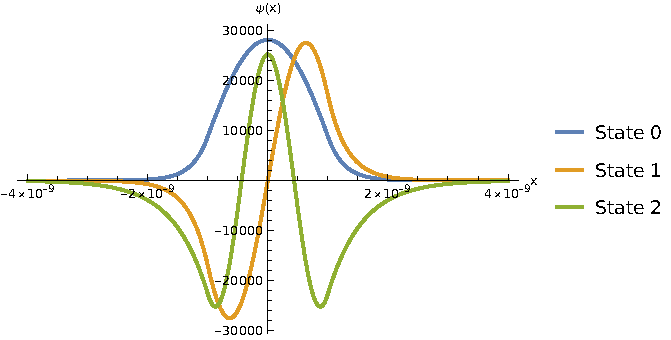
\includegraphics[width=0.6\textwidth]{wavefunctions.pdf}}
\end{figure}
\end{document}